% CVPR 2022 Paper Template
% based on the CVPR template provided by Ming-Ming Cheng (https://github.com/MCG-NKU/CVPR_Template)
% modified and extended by Stefan Roth (stefan.roth@NOSPAMtu-darmstadt.de)

\documentclass[10pt,twocolumn,letterpaper]{article}

%%%%%%%%% PAPER TYPE  - PLEASE UPDATE FOR FINAL VERSION
%\usepackage[review]{cvpr}      % To produce the REVIEW version
\usepackage{cvpr}              % To produce the CAMERA-READY version
%\usepackage[pagenumbers]{cvpr} % To force page numbers, e.g. for an arXiv version

% Include other packages here, before hyperref.
\usepackage{graphicx}
\usepackage{amsmath}
\usepackage{amssymb}
\usepackage{booktabs}
\usepackage{breqn}


% It is strongly recommended to use hyperref, especially for the review version.
% hyperref with option pagebackref eases the reviewers' job.
% Please disable hyperref *only* if you encounter grave issues, e.g. with the
% file validation for the camera-ready version.
%
% If you comment hyperref and then uncomment it, you should delete
% ReviewTempalte.aux before re-running LaTeX.
% (Or just hit 'q' on the first LaTeX run, let it finish, and you
%  should be clear).
\usepackage[pagebackref,breaklinks,colorlinks]{hyperref}


% Support for easy cross-referencing
\usepackage[capitalize]{cleveref}
\crefname{section}{Sec.}{Secs.}
\Crefname{section}{Section}{Sections}
\Crefname{table}{Table}{Tables}
\crefname{table}{Tab.}{Tabs.}


%%%%%%%%% PAPER ID  - PLEASE UPDATE
\def\cvprPaperID{*****} % *** Enter the CVPR Paper ID here
\def\confName{CVPR}
\def\confYear{2022}


\begin{document}

%%%%%%%%% TITLE - PLEASE UPDATE
\title{21  - Preliminary Project Report}

\author{Krishna Srikar Durbha\\
{\tt\small ee18btech11014@iith.ac.in}
% For a paper whose authors are all at the same institution,
% omit the following lines up until the closing ``}''.
% Additional authors and addresses can be added with ``\and'',
% just like the second author.
% To save space, use either the email address or home page, not both
\and
Lakshmi Narasimha Reddy Veluvarthi\\
{\tt\small ee18btech11046@iith.ac.in}
\and
Varun Shankar Moparthi\\
{\tt\small ee18btech11030@iith.ac.in}
\and
Vivek Devara\\
{\tt\small es18btech11024@iith.ac.in}
}
\maketitle

%%%%%%%%% ABSTRACT
\begin{abstract}
In recent years, convolutional neural networks (CNNs) have been copiously applied in various image recognition and processing problems giving state-of-the-art results close to the human-level performance. However, their performance is challenged by the emergence of adversarial machine learning techniques, which could launch powerful attacks on state-of-the-art models. Our work explores the field of classification of videos using deep learning models. We alos explore the vulnerabilty of video classification models for single-frame image noises which is an ascept of electronic noise. We will try to design adversarial attacks at the frame level and observe the susceptibility of models.
\end{abstract}

%%%%%%%%% BODY TEXT

\section{Introduction}
\label{sec:intro}
Convolutional neural networks (CNNs) are a class of deep neural networks that have become prominent in various computer vision tasks. They perform incredibly in extracting spatial features of visual data of a single image. They have proven to be successful at static image recognition challenges like MNIST, CIFAR and ImageNet. CNN's can automatically learn complex features required for recognition, detection, segmentation, and retrieval using a hierarchy of trainable filters and feature pooling operations. The only downside CNNs have their inability to extract temporal relations between frames of images. Recurrent neural networks (RNNs) are another class of deep neural networks primary used for extracting temporal relations in sequential or time-series data. Video analysis provides more information to recognition tasks as they have a time component through which motion and other information can be used and understood. Analysis of a video requires extracting spatial relations in each frame and temporal relations among frames of video. Previously several architectures which combine convolutional layers, recurrent units or an amalgamtion of both have been explored to solve this problem \cite{abuelhaija2016youtube8m} \cite{ng2015short} are successful in classifying videos and have achieved good results.\\


Image noise is an ascept of eletronic noise which can be produced by circuitry of scanner or digital camera. It affects the brightness and colour information of the images. Image noise can also originate in film grain and in the unavoidable shot noise of an ideal photon detector. Image noise is an undesirable by-product of image capture that obscures the desired information. Adversarial machine learning techniques try to fool the machine learning models by providing a perturbed input that is imperceivable to human eyes but affects the performance of machine learning models. These adversarial exampleas are carefully designed and can fool state-of-the-art models which have already at human-level performance \cite{goodfellow2015explaining}. This vulnerability of machine learning models towards adversarial examples raises a concern regarding their application in security-critical applications. Various adversarial attacks techniques have been designed to generate perturbed adversarial examples. Depending on how an adversarial example is created, the attacks can be classified into two categories. One such class of attacks are white-box attacks which complete access to the model like its architecture, gradients, parameters etc. Another class of attacks are called black-box, which only have access to the output of the model. White-box attacks are considered to be strong and model specific i.e as these attacks are complete information of the model, attack use gradients of model (which are specific tot the model) to create perturbations.

\begin{figure}[!ht]
	\centering
	\includegraphics[width=\columnwidth]{Images/Adversarial-Example.png}
	\caption{An adversarial example generated using FGSM attack with GoogLeNet trained on ImageNet.}
\end{figure}

%------------------------------------------------------------------------

\section{Problem Statement}
\label{sec:problem}
Disturbances in the image are usually an aspect of electronic noise produced by an image sensor or the circuitry of a scanner or digital camera. These disturbances occur naturally during capturing an image that will be pretty visible to the human eye. In some cases, images are intentionally perturbed using adversarial techniques to fool the model into misclassifying them, which are also a security concern. These perturbations are artificial and are carefully generated such that these are invisible to the human eye but are powerful enough to fool the model.\\

Let's assume $x_{1:f}^v$ be a video divided into $f$ frames whcih is given as input to our vidoe classification model. In our problem, we deal with scenarios where:
\begin{itemize}
\setlength\itemsep{0.01em}
\item One of the frames of input $x_{1:f}^v$ is corrupted by image noise and how it effects performance of model.
\item Let $x_{a,{1:f}}^v$ denote adversarial frames of $x_{1:f}^v$ perturbed using FGSM or PGD attack. If one frame is randomly chosen from $x_{a,{1:f}}^v$ and it replaces it corresponding frame from $x_{1:f}^v$, how does it effect model's performance?
\item Scenarios where minimum of the frames of input $x_{1:f}^v$ are adversarially corrupted using sparse $l_{2,1}$ adversarial attack to degrade performance of model.
\end{itemize}

%------------------------------------------------------------------------

\section{Literature Review}
\label{sec:literature}
There are many image classification datasets like ImageNet etc., but not many datasets available for video classifications. Some of the famous datasets are UCF-101, Sports-1M, YouTube-8M etc., Out of these datasets, YouTube-8M is the biggest of them with many terabytes and covers more than 500,000 hours of video. It is not practically possible to handle that much data directly in video format with the current computation power available as video have large no.of frames depending on length of the clip and frames-per-second. Therefore, to learn a global description of the video \cite{abuelhaija2016youtube8m} while maintaining a low computational footprint, we will try processing only one frame per second, feeding the decoded frames into the standard ImageNet models and fetch the ReLu activation of the last hidden layer before the classification layer. At this frame rate, a lot of information about motion in video is lost. So, as a solution, we can try to add explicit motion information in the form of optical flow images computed over adjacent frames as seen in paper \cite{ng2015short}. Thus optical flow allows us to retain some motion information while still capturing global video information. Using optical-flow improves the performance of the model by 1\%-2\%.\\

Then after pre-processing, To classify videos, a naive approach would be to treat video frames as still images and apply CNNs to recognize each frame and average the predictions at the video level. However, since each video frame forms only a a small part of the video’s story, such an approach would be using incomplete information could easily confuse classes, especially if fine-grained distinctions or portions of the video are irrelevant to the action of interest.\\

Therefore, we can see that learning a global video temporal evolution is essential for accurate video classification. This is challenging from a modelling perspective as we have to model variable length videos with a fixed number of parameters. Two approaches have been proposed in \cite{ng2015short} that meet this requirement: feature pooling and recurrent neural networks. The feature pooling networks independently process each frame's motion features, which are then quantized and pooled across time. The resulting vector helps make video-level predictions. The recurrent neural network architecture employed is derived from Long Short Term Memory (LSTM) units. Like feature pooling, LSTM networks also access frame-level feature vectors and learn to integrate information over time. 

%--------------------------------------

\section{Approach}
\label{section:approach}
\subsection{Dataset and Data Preprocessing}
We are using the UCF-101 dataset, which contains 13,320 videos with 101 action classes covering a broad set of activities such as sports, musical instruments, and human-object interaction. We shall consider 30 classes in alphabetical order and 90 videos are used for training and 10 videos are used for testing. As no.of videos for training are relatively less to train the model, we opted for an approach that trains the model robustly as well as increases no.of training examples.\\

Let $x_{1:F}^v$ denote a video with $F$ frames. Video classification problem deals with classifying a video i.e a set of image frames $x_{1:F}^v$ to appropriate action entity $y^{e}$. Let's assume $x_{1:f}^v$ where $f=20$ be a subset of $x_{1:F}^v$ and these frames are randomly selected without effecting their sequence. The advantages of this approach are:
\begin{itemize}
\setlength\itemsep{0.01em}
\item Considering frames not from the start or end of the video, we are giving equal weightage to each second of the video as it can't be firmly decided as the most valuable information can be at the start or end of the video.
\item By not considering frames contiguously, we are decreasing the impact of correlation between the frames which there by forces the model to extract temporal relations in a better way from the frames provided.
\item If a video as $F$ frames and the input provided to the model has $f = 20$ frames. There are ${}^{F}C_{f}$ possible ways in which an input can be generated from a single video. This helps the problem of low training videos.
\end{itemize}
Inorder to maintain uniformity across images, all frames of videos are resized to $(128,128)$. Although this reduces the clarity of the image, this resolution is good enough to make predictions.

\subsection{Model Architecture}
We are using CNN-RNN architecture for classifying videos. Since videos contain dynamic data, the transformation between one frame to another may contain addition information which might be useful for making more accurate predictions. As mentioned earlier CNNs are used to extract spatial relations and RNNs are used to extract temporal context of obtained features. Finally fully-connected laters are used at he end for classification. We have considered models that are trained ImageNet to extract features. GRU units are used in RNN network to capture long-term relations. Since we are using UCF-101 dataset we used GRU architecture which gives better and faster results than LSTM networks for small datasets.

\subsubsection{InceptionNet}
InceptionNetv3 which has high performance on ImageNet dataset is used for extracting spatial features of frames of a video. InceptionNetv3 has acheived 3.58\% top-5 error on an ensemble of 4 models. The main motivation developing of InveptionNet are that, 
\begin{itemize}
\setlength\itemsep{0.01em}
\item Dense connections are expensive
\item Biological systems are sparse
\item Sparsity can be exploited by clustering correlated outputs
\end{itemize}

\subsubsection{GRU Architecture}
Let's assume an input sequence $\mathbf{x}=\left(x_{1}, \ldots, x_{T}\right)$ a standard recurrent neural network computes the hidden vector sequence $\mathbf{h}=\left(h_{1}, \ldots, h_{T}\right)$ and output vector sequence $\mathbf{y}=\left(y_{1}, \ldots, y_{T}\right)$ by iterating the following equations from $t=1$ to $T$ :
\begin{equation}
\begin{aligned}
h_{t} &=\mathcal{H}\left(W_{i h} x_{t}+W_{h h} h_{t-1}+b_{h}\right)
\end{aligned}
\end{equation}
\begin{equation}
\begin{aligned}
y_{t} &=W_{h o} h_{t}+b_{o}
\end{aligned}
\end{equation}

where the $W$ terms denote weight matrices (e.g. $W_{ih}$ is the input-hidden weight matrix), the $b$ terms denote bias vectors (e.g. $b_{h}$ is the hidden bias vector) and $\mathcal{H}$ is the hidden layer activation function, typically the logistic sigmoid function.

Unlike standard RNNs, the gated recurrent units (GRUs) architecture can be considered as variations of LSTM networks with a forget gate (Figure \ref{fig:GRU}). GRU uses, update gate and reset gate. to decide what information should be passed to the output. Thus allowing the model to retain information about long-range temporal information which can be usful for making better predictions. The hidden layer $\mathcal{H}$ of the GRU is computed as follows:
\begin{equation}
    \begin{aligned}
        z_{t} &=\sigma_{g}\left(W_{z} x_{t}+U_{z} h_{t-1}+b_{z}\right)
    \end{aligned}
\end{equation}
\begin{equation}
    \begin{aligned}
        r_{t} &=\sigma_{g}\left(W_{r} x_{t}+U_{r} h_{t-1}+b_{r}\right)
    \end{aligned}
\end{equation}
\begin{equation}
    \begin{aligned}
        \hat{h}_{t} &= tanh\left(W_{h} x_{t}+U_{h}\left(r_{t} \odot h_{t-1}\right)+b_{h}\right)
    \end{aligned}
\end{equation}
\begin{equation}
    \begin{aligned}
        h_{t} &=\left(1-z_{t}\right) \odot h_{t-1}+z_{t} \odot \hat{h}_{t}
    \end{aligned}
\end{equation}
where $x_{t}$, $h_{t}:$, $\hat{h}_{t}$, $z_{t}$ and $r_{t}$ are the input, output, candidate activation, update gate and reset gate vectors. $\sigma_{g}$ is a sigmoid function. We chose a GRU architecture where the output from one layer is the input to the next layer.

\begin{figure}
    \centering
    \includegraphics[scale=0.25]{./Images/GRU.png}
    \caption{GRU architecture}
    \label{fig:GRU}
\end{figure}
\subsection{Image Noise}

\begin{itemize}
\setlength\itemsep{0.1em}
\item \textbf{Gaussian Noise}: The primary source of Gaussian noise in digital images is due to inherent noise of sensor due to the level of illumination and its own temperature.\cite{enwiki:1057073251}
\item \textbf{Salt and Pepper Noise}: It is caused by  analog-to-digital converter errors, bit errors in transmission, etc.\cite{enwiki:1057073251}
\item \textbf{Shot Noise}: It is due to variation in the number of photons sensed at a given exposure level. Thsi noise is known as photon shot noise. There can be an additional shot noise from the dark leakage current in the image sensor which is also called as dark shot noise.\cite{enwiki:1057073251}
\item \textbf{Perioidic Noise}: Electrical dn Electromechanical interference during capturing image is a common source of perioidc noise.\cite{enwiki:1057073251}
\end{itemize}

\begin{figure}
\centering
\begin{subfigure}[b]{0.5\columnwidth}
\includegraphics[width=\columnwidth]{Images/Image.jpg}
\caption{Original Image}
\end{subfigure}

\begin{subfigure}[b]{0.495\columnwidth}
\includegraphics[width=\columnwidth]{Images/Gaussian_Noise.png}
\caption{Gaussian Noise}
\end{subfigure}
\begin{subfigure}[b]{0.495\columnwidth}
\includegraphics[width=\columnwidth]{Images/Salt_and_Pepper_Noise.png}
\caption{Salt and Pepper Noise}
\end{subfigure}

\begin{subfigure}[b]{0.495\columnwidth}
\includegraphics[width=\columnwidth]{Images/Shot_Noise.png}
\caption{Shot Noise}
\end{subfigure}
\begin{subfigure}[b]{0.495\columnwidth}
\includegraphics[width=\columnwidth]{Images/Perioidc_Noise.png}
\caption{Perodic Noise}
\end{subfigure}

\caption{Impact of natural noises of camera like Gaussian, Salt and Pepper, Shot and Periodic noises while capturing an image.}
\end{figure}

\subsection{Adversarial Attacks}
\subsubsection{Fast Gradient Sign Method}
Fast Gradient Sign Method (FGSM) is a white-box adversarial attack used to create adversarial examples in a single step. In order to create adversarial examples loss function is modified in such a way that gradients updated help in creating adversarial examples. The perturbations are calculated as follows:
\begin{align}
\boldsymbol{\eta}=\epsilon \operatorname{sign}\left(\nabla_{\boldsymbol{x}} J(\boldsymbol{\theta}, \boldsymbol{x}, y)\right)
\end{align}

\subsubsection{Projected Gradient Descent}
PGD is also white-box adversarial attack to generate adversarial examples through a multi-iterative process. The basic PGD algorithm on an example $x$ with step-size $\alpha$ simply iterates the updates i.e.,

\subsubsection{Sparse $l_{2,1}$ Adversarial Perturbation}
We considered the algorithm from \cite{wei2018sparse} with small modifications. Let $x_{1:f}^v \in \mathbb{R}^{T \times W \times H \times C}$ denote a clean vi
deo, and $x_{a,{1:f}}^v$ denote its adversarial video, where $T$ is the number of frames, $W,H,C$ are the width, height and channel for a specific frame, respectively. $\mathbf{E} = x_{a,{1:f}}^v - x_{1:f}^v$ is the adversarial perturbations. As corrputing all frames of a video is computational expensive, let us consider a mask $M$ which is a temporal mask on the video to enforce some frames having no perturbations where $M \in \{0,1\}^{T \times W \times H \times C}$. Let $\Theta = \{0,1,2..,T\}$ be the set of frame indices, $\Phi$ is a subset within $\Theta$ having $K$ elements, and $\Psi = \Theta - \Phi$. If $t \in \Phi$ we set, $M_{t} = 0$ and if $t \in \Psi$ we set $M_{t} = 1$, where $M_{t} \in \{0,1\}^{T \times W \times H \times C}$ is the $t$-th frame in $\mathbf{M}$. So the problem of finding adversarial perturbation $\mathbf{E}$ becomes as follows:
\vspace{-0.5 em}
\begin{align}
\arg \min _{\mathbf{E}} \lambda\|\mathbf{M} \cdot \mathbf{E}\|_{p} -  \ell\left(\mathbf{1}_{y^{e}}, J_{\theta}\left(\mathbf{x_{i,{1:f}}^v}+\mathbf{M} \cdot \mathbf{E}\right)\right)
\end{align}
where where $l(,·,)$ is the loss function to measure the difference between the prediction and the ground truth label which is categorical cross entropy. $l_{2,1}$ norm is widely used in sparse coding methods. $\|\mathbf{E}\|_{2,1} = \sum_{t}^{T}\left\|E_{t}\right\|_{2}$ where $E_{t} \in \mathbb{R}^{T \times W \times H \times C}$ is the $t$-th frame in $\mathbf{E}$. $l_{2,1}$ norm apply the $l_{1}$ norm across the frames, and thus, can ensure the sparsity of generated perturbations. \\

Our approach differs from \cite{wei2018sparse} as we are not finding a universal perturbation rather we are create a unique perturbation for each example.
%------------------------------------------------------------------------

\section{Results}
GitHub Link for Codes:\\
\href{https://github.com/dks2000dks/Video-Classification}{https://github.com/dks2000dks/Video-Classification}
\subsection{Video Classification}
The classification model is trained with Adam optimizer for $10$ epochs with a batch-size of $256$ and the loss function is set to categorical cross-entropy. Dropout layers are used as a regularization technique inorder to avoid overfitting on training dataset.
\begin{figure}[!ht]
    \centering
    \includegraphics[width=\columnwidth]{./Images/Accuracy.eps}
    \caption{Accuracy vs Epochs}
\end{figure}
\begin{figure}[!ht]
    \centering
    \includegraphics[width=\columnwidth]{./Images/Loss.eps}
    \caption{Accuracy vs Epochs}
\end{figure}
\subsection{Impact of Image Noise}
We assumeing that during capturing a video, perturbations only occur in a single-frame. So, we randomly corrupted a single-frame of the video and observed the performance of the model.
\begin{figure}[!ht]
    \centering
    \includegraphics[width=\columnwidth]{./Images/Image_Noise.eps}
    \caption{Performance of Classification model on Image-Noise.}
\end{figure}
Image-Noise doesn't effect the performance of model. Any single frames natural corruption failed to perturbate the model.

\subsection{Impact of standard Adversarial Attacks}
\begin{figure}[!ht]
    \centering
    \includegraphics[width=0.5\columnwidth]{./Images/FGSM.png}
    \caption{Example of adversarial example generated using FGSM attack}
\end{figure}
\begin{figure}[!ht]
    \centering
    \includegraphics[width=0.5\columnwidth]{./Images/PGD.png}
    \caption{Example of adversarial example generated using PGD attack}
\end{figure}
\begin{figure}[!ht]
    \centering
    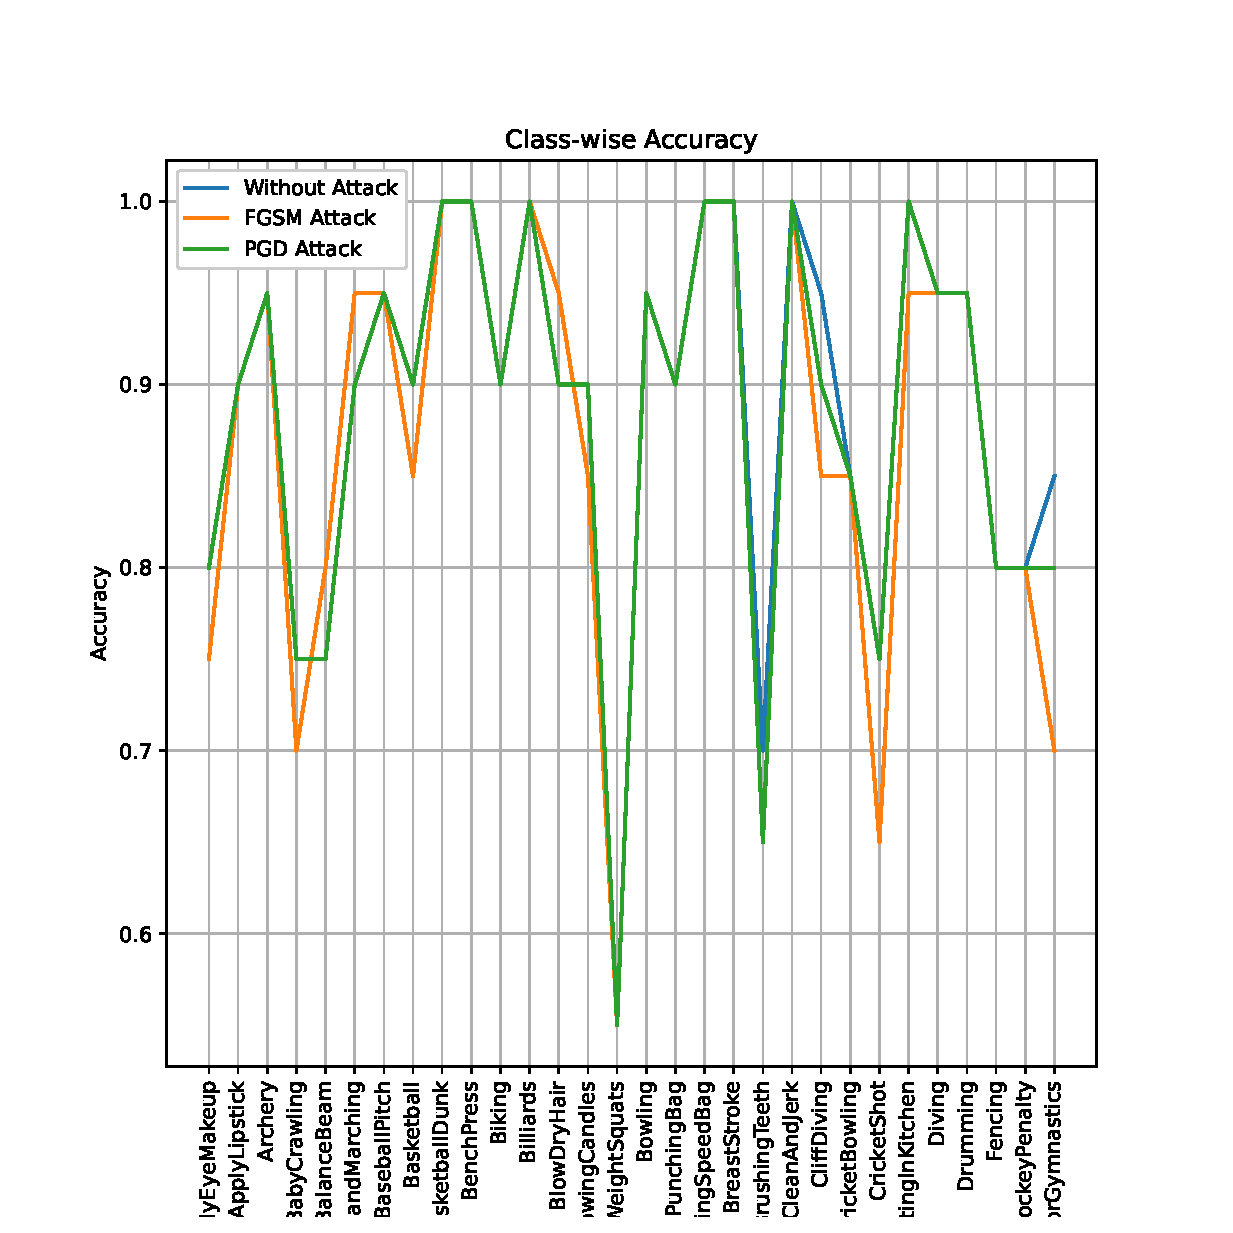
\includegraphics[width=\columnwidth]{./Images/Standard-Adversarial-Attack.eps}
    \caption{Performance of Classification model on FGSM and PGD generated adversarial examples.}
\end{figure}
No performance difference is observed in model's performance. Model is robust towards simgle frame adversarial attacks.
\subsection{Impact of Sparse $l_{2,1}$ Adversarial Perturbation}
We fixed the frames indices in which corruption is happening. The frame indices to be $[0,4,9,13]$. When a minimum 4 frames are corrupted, the performance of model is drastically decreasing.
\begin{figure}[!ht]
    \centering
    \includegraphics[width=0.5\columnwidth]{./Images/Adversarial-Attack.png}
    \caption{Example of adversarial example generated using impact of Sparse $l_{2,1}$ Adversarial Perturbation}
\end{figure}
\begin{figure}[!ht]
    \centering
    \includegraphics[width=\columnwidth]{./Images/Adversarial-Attack.eps}
    \caption{Performance on model on impact of Sparse $l_{2,1}$ adversarial perturbations}
\end{figure}

%-------------------------------------------------------------------------

%%%%%%%%% REFERENCES
{\small
\bibliographystyle{ieee_fullname}
\bibliography{egbib.bib}
}

\end{document}
